\chapter*{Le plus court chemin}

Voici un problème à plusieurs millions! C'est très sérieux: résolvez ce
problème, et vous serez riches et célèbres. Mais malheureusement, c'est un moyen
plutôt compliqué de devenir riche.

\bigskip
\begin{wrapfigure}{r}{0.4\linewidth}
  \vspace{-\baselineskip}
  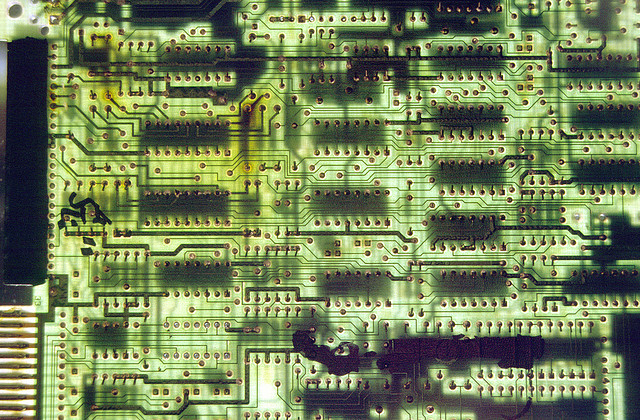
\includegraphics[width=\linewidth]{algo/tsp/electric_city.jpg}
  \vspace{-2\baselineskip}
  \label{img:electric:city}
\end{wrapfigure}
%\begin{center}
%\end{center}

Imaginez que vous fabriquiez des circuits électroniques, comme des téléviseurs.
Pour souder les compsants sur le circuit, il faut percer des trous dans votre
plaque de PCB. Pour cela, un robot doté d'une perceuse va d'un emplacement à
l'autre pour faire les trous.

\medskip
On sent bien que si on s'y prend mal, la tête fait trop de déplacements et perd
du temps, donc de l'argent. En revanche, on voit beaucoup moins bien comment
trouver le meilleur chemin possible\ldots

\encart{Matériel}{
  \begin{itemize}
  \item Une planche plantée de clous, disposés au hasard,
%  \item autant de longs clous que de trous,
  \item une ficelle suffisamment longue (et pas trop élastique),%\textbf{qui ne soit pas élastique},
  \item un marqueur (pour marquer sur la ficelle la longueur du chemin)
  \end{itemize}
}

Le but du jeu est de trouver le plus court chemin passant une fois et une seule
par chaque clou et terminant sur le clou de départ (la perceuse doit être prête
pour la prochaine plaque). On attache une ficelle à un clou et on fait passer la
ficelle de clou en clou, en bouclant.

\bigskip
Parviendrez-vous à trouver le plus court chemin ?

\newpage

\section*{Recherche de la solution optimale}

Ce problème a de nombreuses applications dans la vie de tous les jours :
minimiser la tournée du facteur, la longueur des pistes d'un circuit imprimé,
les déplacements d'un bras robotiquex{\ldots} C'est un problème très étudié,
plus connu sous le nom de \textbf{\og problème du voyageur de commerce \fg}.

Le problème du voyageur de commerce appartient à une catégorie de problèmes très
difficiles à résoudre. Pour ces problèmes, on ne dispose pas d'algorithmes assez
performants pour le résoudre quand $n$ est élevé. Le problème du voyageur de
commerce ayant fait l'objet de nombreuses études, beaucoup d'algorithmes ont été
proposés pour le résoudre le plus efficacement possible.

\subsection*{Comparaison de deux algorithmes}

L'approche naïve consiste à calculer la longueur de tous les chemins possibles,
et comparer les résultats pour ne retenir que le plus court. Pour $n$ villes, le
nombre de chemins possible est $n!$. La performance de l'algorithme est donc
$O(n!)$.

Il existe cependant des algorithmes plus efficaces : par exemple, la performance
de l'algorithme Held-Karp est $O(n^{2}2^n)$. Pour illustrer la différence,
comparons l'augmentation des calculs nécessaires à mesure que $n$ augmente :

\begin{center}
  \begin{tabular}{|l|llll|}
    \hline
    Nombre de sommets       & $5$   & $10$      & $15$            & $20$ \\
    \hline
    %Méthode naïve $O(n!)$   & 120 & 3628800 & 1307674368000 & 2432902008176640000 \\
    %Held-Karp $O(n^{2}2^n)$ & 800 & 102400  & 7372800       & 419430400 \\
    Méthode naïve $O(n!)$   & $120$ & $3628800$ & $1.3 \times 10^{12}$ & $2.4 \times 10^{18}$ \\
    Held-Karp $O(n^{2}2^n)$ & $800$ & $102400$  & $7.3 \times 10^6$       & $4.1 \times 10^8$ \\
    \hline
  \end{tabular} 
\end{center}

Ce tableau indique qu'en testant un milliard de chemins par seconde, il faudrait
à la méthode naïve plus de \textbf{77 ans} pour trouver le chemin le plus court
entre 20 sommets ! Dans les mêmes conditions, l'algorithme Held-Karp met moins
d'\textbf{une demi-seconde} pour trouver le même résultat.

\begin{center}
  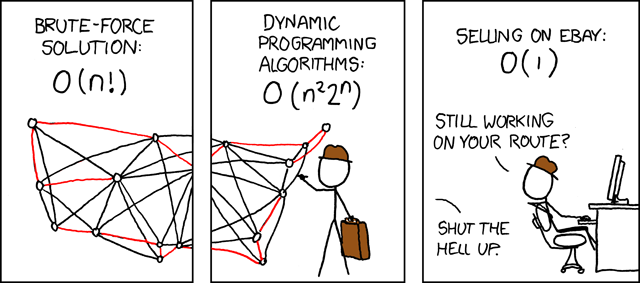
\includegraphics[width=\linewidth]{algo/tsp/tsp_xkcd.png}
  \label{img:tsp_xkcd}
\end{center}

\section*{Recherche d'une solution approchée}

Pour ces problèmes complexes, on préfère souvent trouver une solution
raisonnablement bonne (solution approchée) très rapidement, plutôt que de
chercher très longtemps la solution optimale. Une \textbf{heuristique} est une
méthode pour fouiller intelligemment l'espace des solutions possibles à la
recherche des bonnes solutions. La recherche d'heuristiques efficaces fait
partie du travail des chercheurs en informatique.

\subsection*{Heuristique : le plus proche voisin}

Partez d'une ville, et allez vers la ville la plus proche par laquelle vous
n'êtes pas encore passé. Recommencez, jusqu'à passer par toutes les villes, et
revenez au point de départ. Cette heuristique aura tendance à prendre de
préférence les distances les plus courtes{\ldots} Mais elle n'aboutira pas
forcément à la meilleure solution. Par exemple :

\begin{center}
  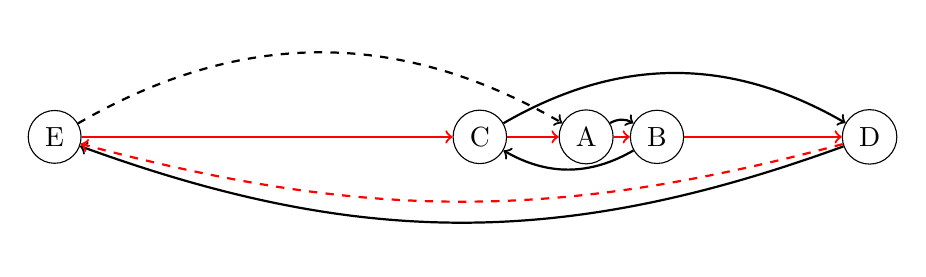
\begin{tikzpicture}[scale=0.45,point/.style={shape=circle,draw}]

%\draw [step=1,thin,color=gray] (-16,-3) grid (9,3);

\node [point] 	(A) at (0,0) {A};
\node [point] 	(B) at (2,0) {B};
\node [point] 	(C) at (-3,0) {C};
\node [point] 	(D) at (8,0) {D};
\node [point] 	(E) at (-15,0) {E};

\draw [thick,->] (A) to [bend left=30] (B);
\draw [thick,->] (B) to [bend left=30] (C);
\draw [thick,->] (C) to [bend left=30] (D);
\draw [thick,->] (D) to [bend left=20] (E);
\draw [thick,->,dashed] (E) to [bend left=30] (A);

\draw [thick,->,color=red] (E) to (C);
\draw [thick,->,color=red] (C) to (A);
\draw [thick,->,color=red] (A) to (B);
\draw [thick,->,color=red] (B) to (D);
\draw [thick,->,color=red,dashed] (D) to [bend left=15] (E);

\end{tikzpicture}

\end{center}

Si on démarre de \tikz \node [shape=circle,draw] {A};, aller toujours vers le
voisin le plus proche nous fait faire un trajet (\tikz \draw[->](0,0) --
(0.5,0);) beaucoup plus long que le trajet optimal (\tikz \draw [->,color=red]
(0,0) -- (0.5,0);).

\subsection*{Heuristiques et méta-heuristiques}

Une heuristique est spécifique au problème qu'elle traite : elle exploite
certaines propriétés du problème pour orienter la recherche vers des \og régions
\fg susceptibles de contenir des bonnes solutions. Cependant, certaines
heuristiques reposent sur des concepts assez génériques pour s'appliquer à de
nombreux problèmes, moyennant quelques adaptations. On parle alors de
\textbf{méta-heuristiques}. Les méta-heuristiques sont souvent inspirées de la
nature. En voici quelques exemples.

\begin{description}
\item[Le recuit-simulé] s'inspire d'un processus utilisé en métallurgie pour
  minimiser l'énergie d'un matériau.
\item[Les colonies de fourmis] s'inspirent du comportement des insectes sociaux
  : avez-vous remarqué que les fourmis finissent toujours par trouver le chemin
  le plus court entre la fourmilière et la source de nourriture ?
\item[Les algorithmes génétiques] reproduisent les mécanismes de l'évolution
  dans le vivant :
  \begin{itemize}
  \item une population de solutions aléatoires est créée ;
  \item on soumet cette population à une sélection naturelle (les meilleures
    solutions sont les plus adaptées) ;
  \item on crée de nouvelles solutions à partir des solutions existantes par
    croisements et mutations ;
  \end{itemize}
  Génération après génération, on observe une amélioration des solutions.
\end{description}

\section*{Le coin de l'animateur}

L'objectif de cette activité est d'introduire la notion de complexité des
problèmes.

\begin{itemize}
\item Commencez par donner un exemple de chemin, en faisant volontairement des
  détours. Laissez ensuite les participants trouver de meilleures solutions.
\item À mesure qu'ils avancent, il sera de plus en plus difficile d'améliorer
  les résultats. Insistez sur le fait que lorsqu'ils trouvent une meilleure
  solution, ils ne peuvent pas être sûrs qu'il n'en existe pas une meilleure.
\item Pour qu'ils se fassent une idée de la complexité du problème, vous pouvez
  demander aux participants de calculer le nombre de chemins possibles ($n!$),
  et les amener à refaire l'estimation du temps de calcul nécessaire à raison
  d'un milliard de chemins testés par seconde.
\end{itemize}

